\begin{boxD}
پیاده‌سازی یک روش نشان‌گذاری از نوع
\grayBox{\lr{Visible}}
و شکننده.

البته بدیهی است که ابتدا باید تحقیق 
کنید و یک روش نشان‌گذاری از نوع 
\grayBox{\lr{Visible}}
و شکننده را پیدا کنید و سپس آن را پیاده سازی کنید.

پیاده‌سازی باید به زبان‌های 
\grayBox{\lr{C++}}
یا 
\grayBox{\lr{Python}}
باشد.‫‪
‬‬
\end{boxD}

\begin{boxA}
ما برای ایجاد یک 
\grayBox{\lr{watermark}}
بر روی تصویر شهید حاج قاسم سلیمانی 
از کتابخانه معروف پردازش تصویر پایتون استفاده کردیم.

ما از کتابخانه
\grayBox{\lr{PIL}}
برای نوشتن متن مدنظر برای 
\grayBox{\lr{watermark}}
شدن استفاده خواهیم کرد.


جمله‌ی مدنظرما برای انتقال به وسیله این تصویر
\newline
\grayBox{\lr{The opportunity that exists}}
        \newline
\grayBox{\lr{ in crises can not be found}} 
        \newline
\grayBox{\lr{  in the opportunities }}
        \newline 
\grayBox{\lr{ themselves !!}}
می‌باشد.
\newline
که ترجمه جمله معروف ایشان مبنی بر فرصتی که در بحران‌ها هست در خود فرصت‌ها نیست.
\end{boxA}


\begin{figure}[h]
    \centering
    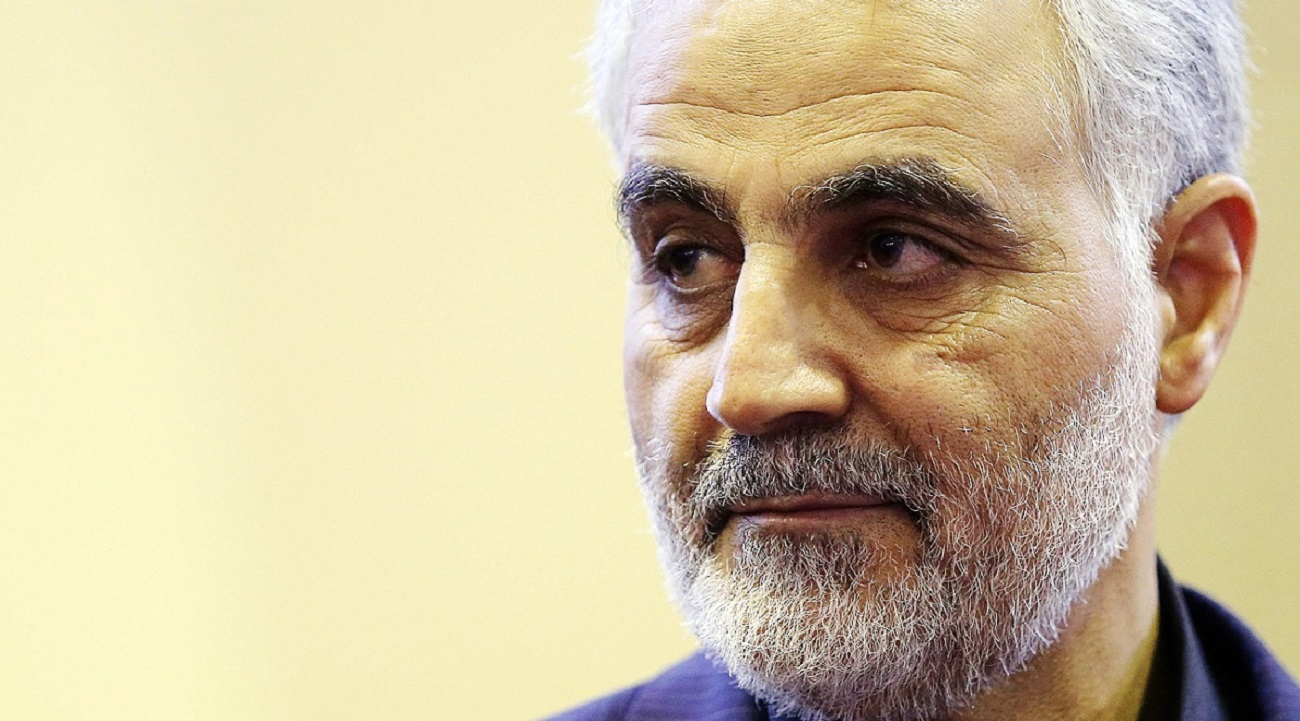
\includegraphics[width=0.85\textwidth]{security_images/sardar2.jpg}
    \caption{تصویر بدون
    \grayBox{\lr{watermark}}}
    % \label{fig:mesh1}
\end{figure}

\begin{figure}[h]
    \centering
    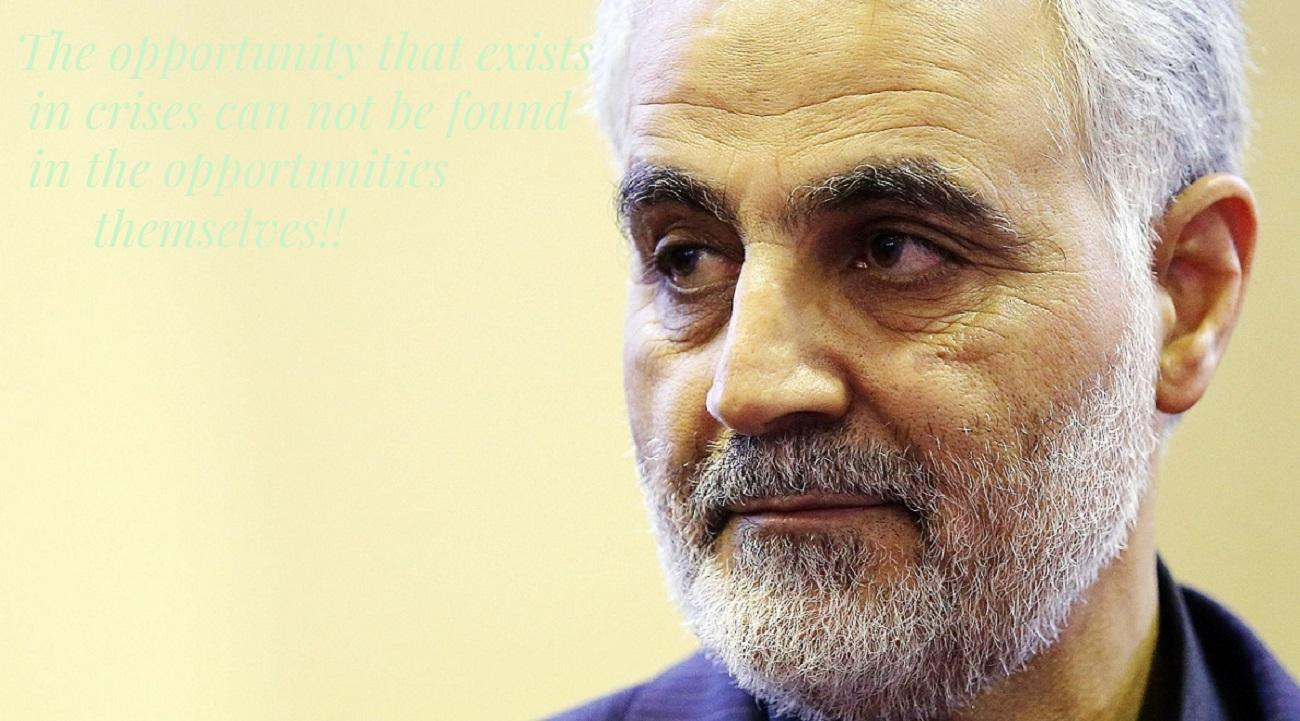
\includegraphics[width=0.85\textwidth]{security_images/result_tmp.jpg}
    \caption{تصویر با شفافیت بیشتر
    \grayBox{\lr{watermark}}}
    % \label{fig:mesh1}
\end{figure}


\begin{figure}[h]
    \centering
    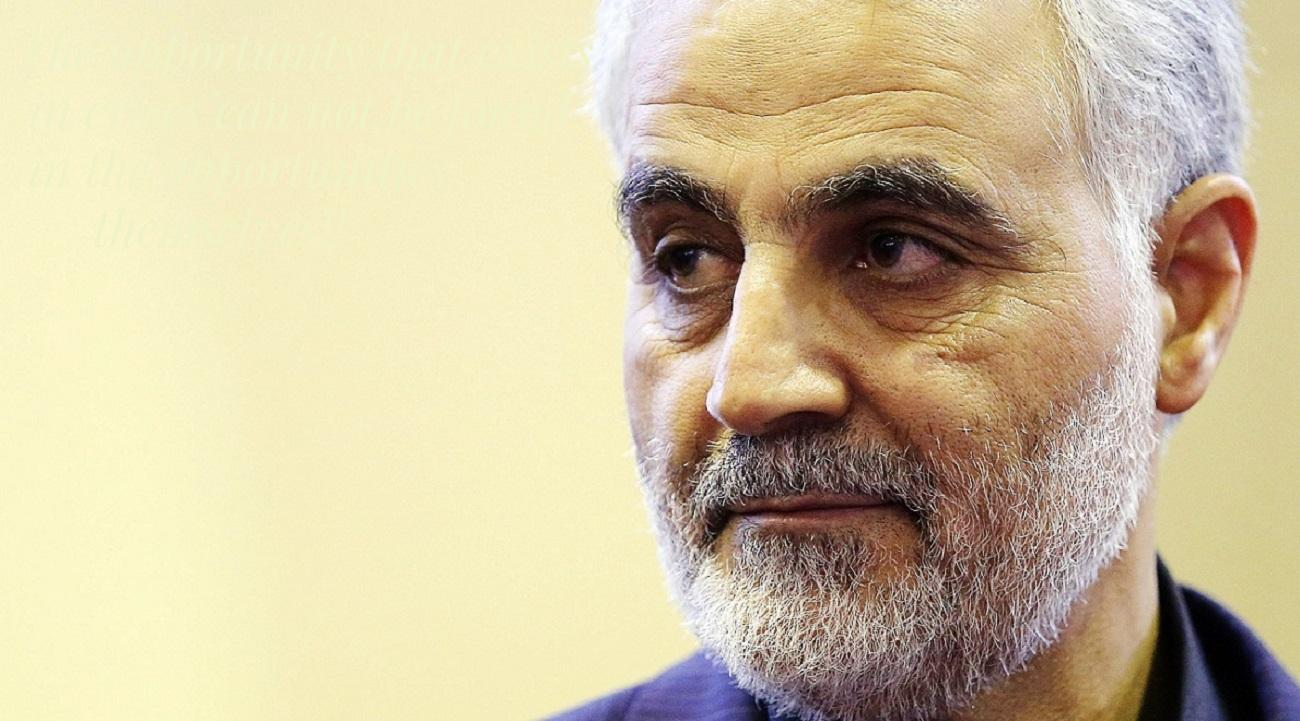
\includegraphics[width=0.85\textwidth]{security_images/result.jpg}
    \caption{تصویر با شفافیت کمتر
    \grayBox{\lr{watermark}}}
    % \label{fig:mesh1}
\end{figure}

\clearpage

\begin{boxA}
    کد مربوط به این 
    \grayBox{\lr{watermark}}
    ها را در زیر مشاهده خواهید کرد.
\end{boxA}

\begin{boxE}
    \lr{\lstinputlisting[language=Python]{security_images/watermark.py}}
\end{boxE}


